\section{Implementation details}
\label{sec:implementation}
In this section, we present extensive experiments to evaluate our proposal. We consider two localisation scenarios: indoor static scenes (section~\ref{subseq:indoor}) and outdoor dynamic scenes (section~\ref{subseq:outdoor}). We also divide our evaluation according to the data available to train our encoder/decoder architecture: fully supervised depth from monocular training (when ground-truth associated depth map are available during training), and unsupervised depth from monocular (when the only data available during training are video sequences with true relative poses between images).

\subsection{Datasets.} We test our method on the following indoor localization datasets: 7 scenes~\citep{Shotton2013} and 12 scenes~\citep{Valentin2016}. These datasets are composed of various indoor environments scanned with RGB-D sensors.  6-DoF image poses and camera calibration parameters are provided for these 2 datasets. For all the experiments, reference images used for the initial pose estimation with \ac{vbl} are taken from the training split and query images are taken from the testing split of the respective datasets.

\subsection{Networks architecture and training.} We use a U-Net like convolutional encoder/decoder architecture~\citep{Isola2017} with multi-scale outputs~\citep{Godard2017}. We denote the fully convolutional architecture as \textbf{FC} and convolutional layers + recurrent layers architecture as \textbf{C+LSTM}. FC and C+LSTM encoders are identical, with 6.3M parameters, FC decoder has 16.7M parameters and C+LSTM decoder has 10.1M parameters.

During training and testing, images are resized to $224 \times 224$ pixels for indoor scenes, and $224 \times 112$ for outdoor images. The generated depth map is 4 times smaller than the RGB input. We use $L_1$ loss function for the fully supervised depth from monocular training. We train our architecture with Adam optimizer, learning rate of $10^{-4}$ divided by two every 50 epochs. Training takes approximately one day on our Nvidia Titan X GPU with a batch size is set to 24.

We train networks for indoor localisation on the 7 scenes dataset (using only sequences from the training split). The 12 scenes dataset is used to evaluate the generalisation capability of our method. For outdoor localisation, we train our two different architectures (FC and C+LSTM) on the Cambridge Landmarks dataset.

\subsection{Method parameters.} We use NetVLAD layer with 64 clusters as global image descriptor for initial pose estimation. We concatenate features from the last convolutional layers of the encoder network, composed of 256 convolutional filters, resulting in a global descriptor of size 16384. Descriptor dimension can be further reduced with PCA projection~\citep{Arandjelovic2017}. We consider the 5-top retrieved candidates from the nearest neighbour search in the pose refinement process, resulting in a good trade-off between time consumption and pose estimation performances. For the final pose estimation, we use the fast \texttt{C++} PnP implementation from~\citep{Kneip2014opengv} and we set the inlier ratio threshold mentioned in section~\ref{subsec:pnlp} to 10\%.
% Local feature for the dense matching between query image and retrieved candidates are extracted from the second convolutional layer of the encoder, resulting on 64-dimensions local descriptors.
\subsection{\acs{iclp} vs \acs{pnlp}.} 

\begin{figure}
\centering

\begin{footnotesize}
\renewcommand{\arraystretch}{1.1}
\newcolumntype{Y}{>{\centering\arraybackslash}X}

\begin{tabularx}{\linewidth}{l | l | c c | Y c c | c c}
			&	Vol.		&	\multicolumn{2}{c|}{\textbf{Only Indexing}}	&  \multicolumn{3}{c|}{\textbf{Scene specific} (one network trained by scene)} 	& \multicolumn{2}{c}{\textbf{All scenes}} \\
%	\cline{3-8} 
	Scene 	&	($m^3$)	&	MAC (M)		  & NetVLAD (V)		& M + ICP w/o dc. &	M + ICP & V + ICP & V + ICP & V + ICP (GT) \\
	\hline
	\hline	
	Chess 	& $6$	&	$0.31m, 14.9^{\circ}$	&	$0.29m, 13.0^{\circ}$	& $0.28m, \ 8.6^{\circ}$		&	$0.23m, \ 5.4^{\circ}$	&	$0.22m, \ 4.9^{\circ}$ &	$0.24m, \ 5.0^{\circ}$		&	$\mathbf{0.12m,\ 4.5^{\circ}}$		\\
	Fire	& $2.5$	&	$0.49m, 16.7^{\circ}$	&	$0.40m, 15.5^{\circ}$	&	$0.39m, 16.5^{\circ}$		& $0.30m, 14.1^{\circ}$	&	$0.30m, 14.1^{\circ}$	 &	$0.26m, \ 9.7^{\circ}$	&	$\mathbf{0.25m,\ 8.9^{\circ}}$	\\
	Heads	& $1$	&	$0.28m, 20.5^{\circ}$   &	$0.20m, 16.0^{\circ}$		&	$0.18m, 14.9^{\circ}$	&	$0.19m, 14.1^{\circ}$	&	$0.17m, 12,9^{\circ}$	&	$\mathbf{0.16m}, 10.1^{\circ}$	&	$0.18m,\ \mathbf{9.9^{\circ}}$	\\
	Office  & $7.5$	&	$0.46m, 16.4^{\circ}$	&	$0.38m, 13.0^{\circ}$		&	$0.41m, 13.4^{\circ}$	& $0.36m, 11.3^{\circ}$		&	$0.30m, \ 8.6^{\circ}$	&	$0.32m, \ 7.8^{\circ}$		&	$\mathbf{0.22m,\ 7.3^{\circ}}$	\\
	Pumpkin & $5$	&	$0.50m, 15.0^{\circ}$	&	$0.43m, 13.1^{\circ}$		&	$0.40m, 12.0^{\circ}$	&	$0.35m, \ 7.4^{\circ}$		&	$0.34m, \ 6.8^{\circ}$	&	$0.37m, \ 6.9^{\circ}$	&	$\mathbf{0.21m,\ 6.2^{\circ}}$	\\
	Red Kitchen & $18$	& $0.30m, 11.2^{\circ}$		&	$0.23m, \ 9.5^{\circ}$		&	$0.24m, \ 7.5^{\circ}$	&	$0.19m, \ 4.9^{\circ}$		&	$0.18m, \ 4.6^{\circ}$	&	$0.23m, \ 5.0^{\circ}$	&	$\mathbf{0.15m,\ 4.5^{\circ}}$	\\
	Stairs  & $7.5$	&	$0.64m, 16.0^{\circ}$		&	$\mathbf{0.46m}, 14.9^{\circ}$		&	$0.57m, 12.2^{\circ}$	&	$0.48m, 10.3^{\circ}$		&	$0.50m, \ \mathbf{9.5^{\circ}}$	&	$0.51m, 10.4^{\circ}$	&	$0.48m, 12.2^{\circ}$	\\
	\hline
	\multicolumn{2}{c|}{\textbf{Complete}} &	$0.40m, 14.8^{\circ}$		&	$0.33m, 12.6^{\circ}$		&	$0.34m, 11.3^{\circ}$	&	$0.28m, \ 8.7^{\circ}$		&	$0.26m, \ 7.7^{\circ}$	&	$0.28m, \ 7.1^{\circ}$  &	$\mathbf{0.20m,\ 6.6^{\circ}}$	\\
\end{tabularx}
\end{footnotesize}

\end{figure}

\begin{figure}
    \centering
    	
   	\begin{minipage}{0.65\linewidth}		
   		\begin{minipage}{0.5\linewidth}
   			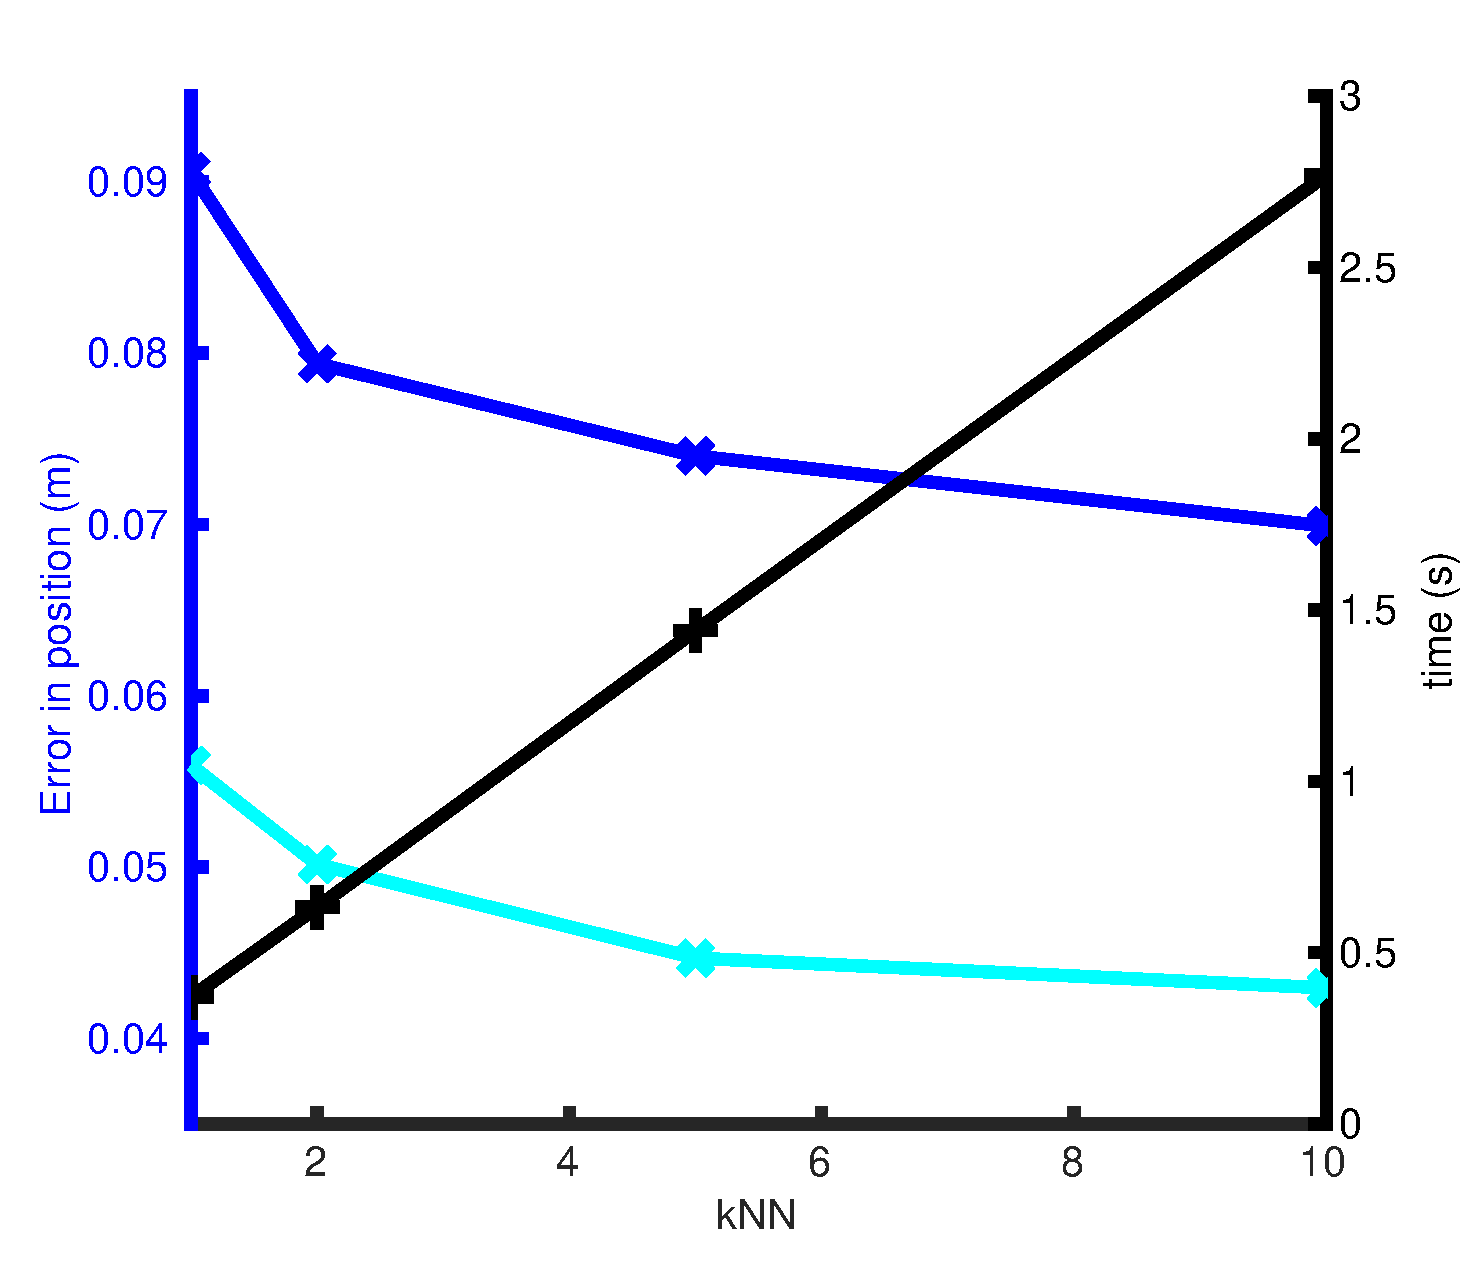
\includegraphics[width=\linewidth]{results/pos_err}
   		\end{minipage}\hfill
   		\begin{minipage}{0.5\linewidth}
   			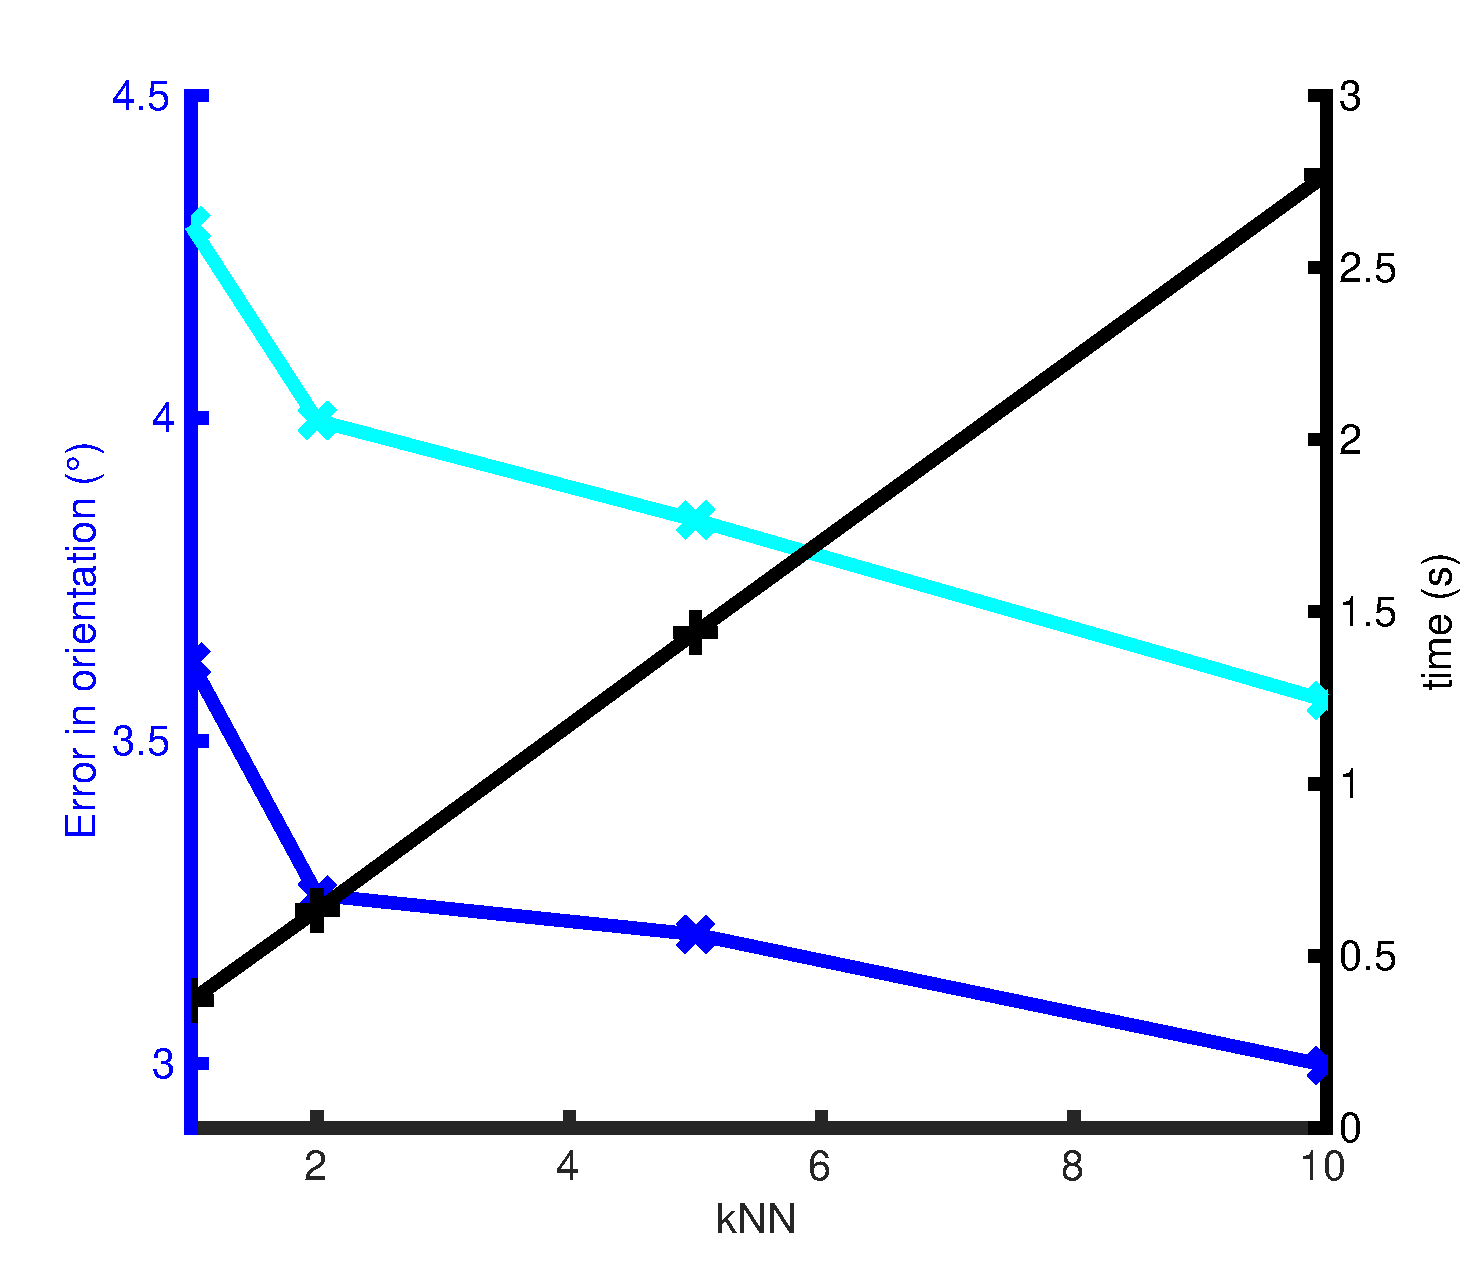
\includegraphics[width=\linewidth]{results/ori_err}
   		\end{minipage}
   		
   		\vspace{0.2cm}
   		
   		\begin{footnotesize}
   			\setlength{\tabcolsep}{2pt}
   			\begin{tabular}{c l c l c l}
   				\textcolor{red}{\Large{- -}} & NetVALD + RGB & \textcolor{blue}{\Large{- -}} & NetVALD + RGB(D)  & \textcolor{magenta}{\Large{- -}} & NetVALD + RGB(H)\\
   				\textcolor{red}{\Large{--}} & MAC + RGB & \textcolor{blue}{\Large{--}} & MAC + RGB(D) & \textcolor{magenta}{\Large{--}} & MAC + RGB(H)\\
   			\end{tabular}		
   		\end{footnotesize}
   		
   	\end{minipage}\hfill
   	\begin{minipage}{0.35\linewidth}
   		\caption[]{\label{fig:ratio_t_knn} .}
   	\end{minipage}	
	
	
	
\end{figure}